\chapter{The Ethernet Model}
\label{cha:ethernet}

TODO EtherMacFullDuplex --> EtherMac
TODO EtherMac --> EtherCsmaCdMac
TODO there is no IWiredNic with EtherLLC
TODO: model delay in hubs: class I device 140 bit time, class II device 92 bit time (for fast ethernet)

\section{Overview}

Ethernet is the most popular wired LAN technology nowadays, also used in
metropolitan area and wide area networks.

Variations: 10Mb/s ethernet, fast ethernet, Gigabit Ethernet, Fast Gigabit Ethernet, full duplex

TODO: 802.1d (STP, RSTP), 802.2 (LLC), ...


\section{Nodes}

\begin{itemize}
  \item Node models such as \nedtype{StandardHost} and \nedtype{Router} are Ethernet-capable
  \item \nedtype{EtherSwitch} TODO switching hub
  \item \nedtype{EtherHub} TODO repeating hub
  \item \nedtype{EtherBus} TODO legacy coaxial cable
  \item \nedtype{EtherHost} TODO is a sample node
\end{itemize}

how to connect networks

how to add stp/rstp

TODO describe PAUSE handling here

\subsection{EtherSwitch}

Ethernet switches play an important role in modern Ethernet LANs. Unlike
passive hubs and repeaters, that work in the physical layer, the switches
operate in the data link layer and routes data frames between the connected
subnets.

While a hub repeats the data frames on each connected line, possibly causing
collisions, switches help to segment the network to small collision domains.
In modern Gigabit LANs each node is connected to the switch direclty
by full-duplex lines, so no collisions are possible. In this case the
CSMA/CD is not needed and the channel utilization can be high.

\nedtype{EtherSwitch} models an Ethernet switch.

The duplexChannel attributes of the MACs must be set according to the
medium connected to the port; if collisions are possible (it's a bus or hub)
it must be set to false, otherwise it can be set to true.
By default it uses half duples MAC with CSMA/CD.

TODO STP, RSTP

\subsection{EtherHub}

Ethernet hubs are a simple broadcast devices. Messages arriving on a port
are regenerated and broadcast to every other port.

The connections connected to the hub must have the same data rate.
Cable lengths should be reflected in the delays of the connections.

Messages are not interpreted by the \nedtype{EtherType} hub model in any way,
thus the hub model is not specific to Ethernet. Messages may
represent anything, from the beginning of a frame transmission to
end (or abortion) of transmission.



\subsection{EtherBus}

The \nedtype{EtherBus} component can model a common coaxial cable
found in early Ethernet LANs. The nodes are attached via taps at specific
positions on the cable. When a node sends a signal, it will propagate
along the cable in both directions at the given propagation speed.

The gates of the \nedtype{EtherBus} represent taps. The positions
of the taps are given by the \fpar{positions} parameter as a
space separated list of distances in metres. If there are more
gates then positions given, the last distance is repeated.
The bus component send the incoming message in one direction and
a copy of the message to the other direction (except at the ends).
The propagation delays are computed from the distances of the taps
and the \fpar{propagationSpeed} parameter.

Messages are not interpreted by the bus model in any way, thus the bus
model is not specific to Ethernet. Messages may represent anything, 
from the beginning of a frame transmission to end (or abortion) of transmission.

% FIXME #356 NED comment is wrong: data rate must not be zero!
% FIXME #354 default propagation speed is wrong (should be 2e8mps)
%            btw there is a hard coded propagation speed in EtherMACBase.cc



\section{Physical layer}

Stations on an Ethernet networks are connected by coaxial,
twisted pair or fibre cables. (Coaxial only has historical importance,
but is supported by INET anyway.) There are several cable types specified
in the standard.

In the INET framework, the cables are represented by connections.
The connections used in Ethernet LANs must be derived from
\nedtype{DatarateConnection} and should have their \fpar{delay} and
\fpar{datarate} parameters set.
The delay parameter can be used to model the distance between the
nodes. The datarate parameter can have four values:

\begin{itemize}
  \item \ttt{10Mbps} classic Ethernet
  \item \ttt{100Mbps} Fast Ethernet
  \item \ttt{1Gbps} Gigabit Ethernet
  \item \ttt{10Gbps} Fast Gigabit Ethernet
\end{itemize}

\section{Ethernet Interfaces}

The \nedtype{EthernetInterface} compound module implements the \nedtype{IWiredInterface}
interface. Complements \nedtype{EtherMac} and \nedtype{EtherEncap} with an output queue
for QoS and RED support. It also has configurable input/output filters as \nedtype{IHook}
components similarly to the \nedtype{PppInterface} module.

The Ethernet MAC (Media Access Control) layer transmits the Ethernet frames on
the physical media. This is a sublayer within the data link layer. Because
encapsulation/decapsulation is not always needed (e.g. switches does not do
encapsulation/decapsulation), it is implemented in a separate modules
(\nedtype{EtherEncap} and \nedtype{EtherLlc}) that are part of the LLC layer.


Nowadays almost all Ethernet networks operate using full-duplex
point-to-point connections between hosts and switches. This means
that there are no collisions, and the behaviour of the MAC component
is much simpler than in classic Ethernet that used coaxial cables and
hubs. The INET framework contains two MAC modules for Ethernet:
the \nedtype{EtherMacFullDuplex} is simpler to understand and easier to extend,
because it supports only full-duplex connections. The \nedtype{EtherMac}
module implements the full MAC functionality including CSMA/CD, it
can operate both half-duplex and full-duplex mode.

\subsection*{Queueing}

When the transmission line is busy, messages received from the upper layer
needs to be queued.

In routers, MAC relies on an external queue module (see \nedtype{OutputQueue}),
and requests packets from this external queue one-by-one. The name of the
external queue must be given as the \fpar{queueModule} parameer.
There are implementations of \nedtype{OutputQueue} to model finite buffer,
QoS and/or RED.

In hosts, no such queue is used, so MAC contains an internal
queue named \fvar{txQueue} to queue up packets waiting for transmission.
Conceptually, \fvar{txQueue} is of infinite size, but for better diagnostics
one can specify a hard limit in the \fpar{txQueueLimit} parameter -- if this is
exceeded, the simulation stops with an error.

\subsection*{PAUSE handling}
\label{subsec:pause_handling}

The 802.3x standard supports PAUSE frames as a means of flow
control. The frame contains a timer value, expressed as a multiple
of 512 bit-times, that specifies how long the transmitter should
remain quiet. If the receiver becomes uncongested before the
transmitter's pause timer expires, the receiver may elect to send
another PAUSE frame to the transmitter with a timer value of zero,
allowing the transmitter to resume immediately.

\nedtype{EtherMac} will properly respond to PAUSE frames it receives
(\msgtype{EtherPauseFrame} class),
however it will never send a PAUSE frame by itself. (For one thing,
it doesn't have an input buffer that can overflow.)

\nedtype{EtherMac}, however, transmits PAUSE frames received by higher layers,
and \nedtype{EtherLlc} can be instructed by a command to send a PAUSE frame to MAC.

% FIXME PAUSE frames should only be sent on full-duplex ethernet.
%       If a switch uses half-duplex mode to connect to hosts, it can ask sending hosts
%       to slow down their sending rates:
%       - force collisions with incoming frames
%       - make it appear as if the channel is busy
% FIXME PAUSE frames should have 0x8808 in the etherType field

\subsection*{Error handling}

If the MAC is not connected to the network ("cable unplugged"), it will
start up in "disabled" mode. A disabled MAC simply discards any messages
it receives. It is currently not supported to dynamically connect/disconnect
a MAC.

CRC checks are modeled by the \fvar{bitError} flag of the packets. Erronous
packets are dropped by the MAC.


%\subsection*{Auto-Negotiation}
% Ethernet Auto-Negotiation not supported


\section{Components}

Thw following components:

\begin{itemize}
  \item \nedtype{EtherMacFullDuplex}
  \item \nedtype{EtherMac}
  \item \nedtype{EtherLlc}
  \item \nedtype{EtherEncap}
  \item \nedtype{MacRelayUnit}
  \item \nedtype{Ieee802dRelay}
\end{itemize}


\subsection{EtherMacFullDuplex}

From the two MAC implementation \nedtype{EtherMacFullDuplex} is the simpler one,
it operates only in full-duplex mode (its \fpar{duplexEnabled} parameter fixed to
\ttt{true} in its NED definition). This module does not need to implement
CSMA/CD, so there is no collision detection, retransmission with exponential backoff,
carrier extension and frame bursting. Flow control works as described in section
\ref{subsec:pause_handling}.

% FIXME remove frameBursting from NED def, or fix it to false
%       currently setting it to 'true' has no effect

In the \nedtype{EtherMacFullDuplex} module,
packets arrived at the \ttt{phys\$i} gate are handled when their last bit received.

Outgoing packets are transmitted according to the following state diagram:

\begin{center}
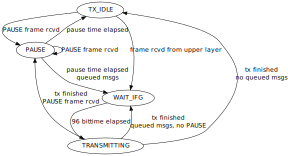
\includegraphics{figures/EtherMACFullDuplex_txstates}
\end{center}

\subsection{EtherMac}

Ethernet MAC layer implementing CSMA/CD. It supports both half-duplex and full-duplex operations;
in full-duplex mode it behaves as \nedtype{EtherMacFullDuplex}. In half-duplex  mode
it detects collisions, sends jam messages and retransmit frames upon collisions using
the exponential backoff algorithm. In Gigabit Ethernet networks it supports carrier
extension and frame bursting. Carrier extension can be turned off by setting the
\fpar{carrierExtension} parameter to \ttt{false}.

Unlike \nedtype{EtherMacFullDuplex}, this MAC module processes the incoming packets when their
first bit is received. The end of the reception is calculated by the MAC and
detected by scheduling a self message.

When frames collide the transmission is aborted -- in this case the transmitting
station transmits a jam signal. Jam signals are represented
by a \msgtype{EtherJam} message. The jam message contains the tree identifier
of the frame whose transmission is aborted. When the \nedtype{EtherMac} receives a jam
signal, it knows that the corresponding transmission ended in jamming and have
been aborted. Thus when it receives as many jams as collided frames, it can
be sure that the channel is free again. (Receiving a jam message marks the
beginning of the jam signal, so actually has to wait for the duration of the jamming.)

The operation of the MAC module can be schematized by the following state chart:

\begin{center}
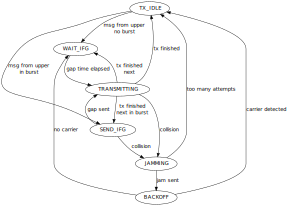
\includegraphics{figures/EtherMAC_txstates}
\end{center}


\subsection{EtherEncap}

The \nedtype{EtherEncap} module generates \msgtype{EthernetIIFrame} messages.

EtherFrameII

\subsection{EtherLlc}

TODO what it does


% document error conditions (causing error() calls in the code)

% FIXME handleRestransmission() comment is not true: // no beginSendFrames(), because end of jam signal sending will trigger it automatically
%       in case of inner queue, the queued msg is not transmitted
% FIXME should not enter PAUSE state when !duplexMode


\subsection{MacRelayUnit}

INET framework ethernet switches are built from \nedtype{IMacRelayUnit}
components. Each relay unit has N input and output gates for sending/receiving
Ethernet frames. They should be connected to \nedtype{IEtherMac} modules.

Internally the relay unit holds a table for the destination address -> output
port mapping. When it receives a data frame it updates the table with the
source address->input port. The table can also be pre-loaded from a text file
while initializing the relay unit. The file name given as the \fpar{addressTableFile}
parameter. Each line of the file contains a hexadecimal MAC address and a decimal port
number separated by tabs. Comment lines beginning with '\#' are also allowed:

\begin{verbatim}
01 ff ff ff ff    0
00-ff-ff-ee-d1    1
0A:AA:BC:DE:FF    2
\end{verbatim}

% FIXME #352 addressTableSize is not checked in readAddressTable -> if overflown
%            then later check updateTableWithAddress has no effect
% FIXME format is wrong in the comment of readAddressTable()

The size of the lookup table is restricted by the \fpar{addressTableSize} parameter.
When the table is full, the oldest address is deleted. Entries are also deleted
if their age exceeds the duration given as the \fpar{agingTime} parameter.

If the destination address is not found in the table, the frame is broadcasted.
The frame is not sent to the same subnet it was received from, because the
target already received the original frame. The only exception if the frame
arrived through a radio channel, in this case the target can be out of range.
The port range 0..\fpar{numWirelessPorts}-1 are reserved for wireless connections.

The \nedtype{IMacRelayUnit} module is not a concrete implementation,
it just defines gates and parameters an \nedtype{IMacRelayUnit} should have.
Concrete inplementations add
capacity and performance aspects to the model (number of frames processed
per second, amount of memory available in the switch, etc.)

There are two versions of \nedtype{IMacRelayUnit}: \nedtype{MacRelayUnit}]

A simple scheme for sending PAUSE frames is built in (although
users will probably change it). When the buffer level goes
above a high watermark, PAUSE frames are sent on all ports.
The watermark and the pause time is configurable; use zero
values to disable the PAUSE feature.

\subsection{Ieee802dRelay}

\nedtype{Ieee802dRelay} ..............


\section{Implemented Standards}

The Ethernet model operates according to the following standards:

\begin{compactitem}
  \item Ethernet: IEEE 802.3-1998
  \item Fast Ethernet: IEEE 802.3u-1995
  \item Full-Duplex Ethernet with Flow Control: IEEE 802.3x-1997
  \item Gigabit Ethernet: IEEE 802.3z-1998
\end{compactitem}

%%% Local Variables:
%%% mode: latex
%%% TeX-master: "usman"
%%% End:
